%
%
%
%

\documentclass{llncs}
\usepackage{graphicx}
\usepackage{booktabs}
\usepackage{latexsym}

\begin{document}

\newcommand\ample{A\textsc{mple} }
\newcommand\gransim{G\textsc{ran}S\textsc{im}}


\title{An AMPLE Implementation}

\author{Ben Lippmeier \and Clem Baker-Finch}

\institute{
	Department of Computer Science \\Australian National University, Canberra, ACT 0200, Australia\\
	\email{Ben.Lippmeier@anu.edu.au, Clem.Baker-Finch@anu.edu.au}}

\maketitle


\begin{abstract}
\ample is an Abstract Machine for Parallel Lazy Evaluation. \ample was created as an experimental environment in which to study the behaviour of lazy functional programs when running on parallel machines with various characteristics. \ample is designed to be highly configurable and all configuration parameters may be set interactively. This configuration extends to the number of processors in the machine, the communication latency and the method used for spawning and unblocking threads. \ample includes tools to generate graphs of profiling data and allows program execution to be traced step by step. \ample has been written entirely in Haskell and has been constructed in a modular way. \ample is intended to be modified by end users in order to investigate their own machine designs.

\end{abstract}



% ------------------------------------------------------------------------------------------------------- Macros
%

\newcommand\rrule[9] {
	\noindent \textbf{#1}
	\par
	\medskip
	\noindent
	\begin{tabular} {p{ 5mm} p{ 2mm} p{20mm} p{25mm} p{15mm} p{ 3mm} p{42mm}}
			& ( & #2, & \raggedleft{#3}, & \raggedleft{#4} & ) & #5\\
	$\Rightarrow$	& ( & #6, & \raggedleft{#7}, & \raggedleft{#8} & ) & #9
	\end{tabular}
	\\
}	


\newcommand\rruleCfSE[9] {
	\noindent \textbf{#1}
	\par
	\medskip
	\noindent
	\begin{tabular} {p{ 5mm} p{ 2mm} p{30mm} p{20mm} p{10mm} p{ 3mm} p{42mm}}
			& ( & #2, & \raggedleft{#3}, & \raggedleft{#4} & ) & #5\\
	$\Rightarrow$	& ( & #6, & \raggedleft{#7}, & \raggedleft{#8} & ) & #9
	\end{tabular}
	\\
}	


\newcommand\rruleCESfH[9] {
	\noindent \textbf{#1}
	\par
	\medskip
	\noindent
	\begin{tabular} {p{ 5mm} p{ 2mm} p{30mm} p{35mm} p{25mm} p{ 3mm} p{5mm}}
			& ( & #2, & \raggedleft{#3}, & \raggedleft{#4} & ) & #5\\
	$\Rightarrow$	& ( & #6, & \raggedleft{#7}, & \raggedleft{#8} & ) & #9
	\end{tabular}
	\\
}	


\newcommand\rruleCEfHS[9] {
	\noindent \textbf{#1}
	\par
	\medskip
	\noindent
	\begin{tabular} {p{ 5mm} p{ 2mm} p{30mm} p{50mm} p{10mm} p{ 3mm} p{5mm}}
			& ( & #2, & \raggedleft{#3}, & \raggedleft{#4} & ) & #5\\
	$\Rightarrow$	& ( & #6, & \raggedleft{#7}, & \raggedleft{#8} & ) & #9
	\end{tabular}
	\\
}	



	
\newcommand\rruleH[9] {
	\noindent \textbf {#1}
	\par
	\medskip
	\noindent
	\begin{tabular} {p{ 5mm} p{40mm} p{ 2mm} p{30mm} p{20mm} p{15mm} p{ 2mm}}	
			& #2 & ( & #3, & \raggedleft{#4}, & \raggedleft{#5} & ) \\
	$\Rightarrow$	& #6 & ( & #7, & \raggedleft{#8}, & \raggedleft{#9} & ) 
	\end{tabular}
	\\
}


\newcommand\rruleHH[9] {
	\noindent \textbf {#1}
	\par
	\medskip
	\noindent
	\begin{tabular} {p{ 5mm} p{50mm} p{ 2mm} p{30mm} p{10mm} p{15mm} p{ 2mm}}	
			& #2 & ( & #3, & \raggedleft{#4}, & \raggedleft{#5} & ) \\
	$\Rightarrow$	& #6 & ( & #7, & \raggedleft{#8}, & \raggedleft{#9} & ) 
	\end{tabular}
	\\
}


\newcommand\rruleE[9] {
	\noindent \textbf {#1}
	\par
	\medskip
	\noindent
	\begin{tabular} {p{ 5mm} p{10mm} p{ 2mm} p{30mm} p{50mm} p{10mm} p{ 2mm}}	
			& #2 & ( & #3, & \raggedleft{#4}, & \raggedleft{#5} & ) \\
	$\Rightarrow$	& #6 & ( & #7, & \raggedleft{#8}, & \raggedleft{#9} & ) 
	\end{tabular}
	\\
}


\newcommand\blocked		{$\Box$}
\newcommand\blackhole		{$\bullet$}
\newcommand\blockedon[1]	{$\bullet \, _{#1}$}
\newcommand\bind		{$\rightarrow \:$}
\newcommand\px			{p$_x$}



% -------------------------------------------------------------------------------------------------------- Introduction
\section{Introduction}
During the design of a system for parallel evaluation it is useful to profile the performance of several archetypal programs. This is done in order to determine whether the decisions taken at design time will lead to the  efficient execution of programs once the system has been implemented. Unfortunately, profiling support is usually something which is added \emph{after} large parts of a system have already been implemented. Although it may be possible to hand-evaluate trivial programs at design time, answering seemingly straight forward questions such as ``How many processors can this program make use of?" is surprisingly hard to do without having access to a good run-time profiler. \cite{loidl:thesis}

One possibility is to make use of an abstract machine in order to profile small programs and test out ideas. By using an abstract machine, important questions regarding the behaviour of a system may be answered without having to build a native implementation. Compared to a native implementation, it is also easier to modify an abstract machine as the design changes and to reason about how it operates.

\ample implements the parallel lazy abstract machine described in \cite{baker-finch:sfp99}. This machine is based on the operational semantics for parallel lazy evaluation given in \cite{baker-finch+king+trinder:icfp2000} as well as Sestoft's derivation of a (sequential) lazy abstract machine \cite{sestoft:abstractmachine}. These are SECD style environment machines which incorporate a model of parallelism consisting of a pool of threads that communicate via a common heap.

Two versions of \ample have been implemented, based on Sestoft's \mbox{Mark-1} and \mbox{Mark-3} machines respectively. The \mbox{Mark-1} machine uses direct substitution to perform function application whereas the \mbox{Mark-3} machine uses a separate environment to model this substitution. The two versions accept a similar source language which differs only in details specific to the abstract machine used. This paper focuses on the version based on Sestoft's \mbox{Mark-3} machine.

\ample implements three different execution modes: single threaded, fully speculative and explicitly parallel. In the single threaded mode a sole thread exists and reductions are performed in a sequential manner. In the fully speculative mode one thread evaluates the function body while a new thread is created to evaluate the argument. In the explicitly parallel mode parallelism is controlled with the \texttt{par} and \texttt{seq} combinators in a manner similar to GpH \cite{trinder:strategies}.

\ample allows configuration parameters to be tuned interactively. This configuration extends to the number of processors in the machine, the communication latency and the method used for spawning and unblocking threads. \ample also provides a rich set of profiling tools that can be used to study the effect that these parameters have on the run-time behaviour of the machine.

\ample has been written entirely in Haskell and has been constructed in a modular way. This modularity is intended to allow the user to modify \ample to meet their own requirements. 


% ------------------------------------------------------------------------------------------------------- Core Language
\section{Core language}
\ample accepts programs written in a small lazy functional language. This language is based on the untyped lambda calculus, augmented with mutually recursive let-bindings, integers, constructors and the \texttt{par} and \texttt{seq} combinators. An abbreviated syntax for this language is shown in figure\,\ref{figSourceSyntax}. The \ample compiler translates program source into the \ample \emph{core} language by converting it to the normalized lambda calculus while replacing variable names with de Bruijn indices as per Sestoft's \mbox{Mark-3} machine. The compiler also builds environment trimmers for let expressions and constructors \cite{sestoft:abstractmachine}.

At run-time the program exists as a graph of `cells' which are stored in a static heap. Each cell is referenced by its offset (pointer) into the heap and the edges of the graph are represented by including these pointers in its cells. 

\begin{figure}
\hrule
\medskip
\begin{tabular}{p{1cm}l}
e  & = \textbf{$\lambda$}x \textbf{.} e 
     $\;|\;$  e$_1$ e$_2$  
     $\;|\;$  x \\
   & $\;|\;$  \textbf{let \{} x$_i$ $\overline{\textrm{y}}_i$ \textbf{=} e$_i$ \textbf{\} in} e \\
   & $\;|\;$  \emph{n} $\;|\;$ e$_1$ \emph{op} e$_2$ \\
   & $\;|\;$  C$_{i}$ $\overline{\textrm{y}}_i$ 
     $\;|\;$  \textbf{case} e \textbf{of \{} C$_i$ $\overline{\textrm{y}}_i$ \textbf{$\rightarrow$} e$_i$ \} \\
   & $\;|\;$  e$_1$ \textbf{par} e$_2$ 
    $\;|\;$  e$_1$ \textbf{seq} e$_2$ \\
\end{tabular}
\medskip
\hrule
\caption{abbreviated syntax for the \ample source language}
\label{figSourceSyntax}
\end{figure}


\section{The AMPLE abstract machine}
The \ample abstract machine is a combination of Sestoft's \mbox{Mark-3} machine \cite{sestoft:abstractmachine} and the Parallel Lazy Abstract Machine described in \cite{baker-finch:sfp99}. The machine is defined by a set of state transition rules, the full set of which is given in the appendix. In single threaded mode the machine operates as per Sestoft's \mbox{Mark-3} machine and the two parallel modes are defined by modifying the set of rules for single threaded mode.


\subsection{Sestoft's Mark-3 machine}
Sestoft's \mbox{Mark-3} machine of consists of a \emph{control} C, an \emph{environment} E, a \emph{stack} S and a \emph{heap} H. 

The control holds the sub-expression currently being evaluated. In the \ample machine the control is a pointer to one of the program cells described in the previous section. Each cell represents one node of the program graph. In this configuration the control is equivalent to the program counter in an imperative machine.

The environment eliminates the need to modify the live program during \mbox{$\beta$\emph{-reduction}}, as is done by Sestoft's \mbox{Mark-1} machine. In the \mbox{Mark-3} machine the environment is a stack of heap pointers $p$. Where the \mbox{Mark-1} machine would perform the direct substitution $e[y/x]$, modifying the original expression $e$, the \mbox{Mark-3} machine inserts $y$ together with a copy of its associated environment into the heap. The resulting heap pointer is then added to the environment for $e$. At compile time each named variable $x$ is replaced by an integer offset into the environment -- so that when the machine requires the value of that variable it can be obtained by following the associated heap pointer.

The heap now maps pointers $p$ onto \emph{closures} $(e, E)$ which represent the result of substituting values referenced by the environment $E$ into the expression $e$. 

The stack represents the context of the evaluation. For example, to evaluate an application $e\:x$ the corresponding heap pointer $p_x$ is pushed onto the stack before proceeding to evaluate $e$ to an abstraction $\lambda e'$. At this point $p$ will be available on the top of the stack and will be 'substituted' into $e'$ by adding it to the current environment. In a similar fashion the stack will hold the case alternatives while a case object is being evaluated, as well as the second argument of \texttt{seq} during the evaluation of the first.

The stack may also contain update markers. When the machine arrives at a variable $x$ an update marker for the associated heap pointer \#$p_x$ is pushed onto the stack. The closure at $p_x$ is then evaluated to whnf, after which the marker indicates that the heap should be updated with this result.

\subsection{Parallel evaluation}
\ample uses a model of parallelism that consists of a set of threads which communicate via a common heap. Each thread contains its own control, environment and stack and is labeled with an index $t$. The transition rules for the appropriate evaluation mode are applied to each thread separately and a given thread becomes inactive when no rule applies. The transition rules are given in the appendix.

\subsection{Fully speculative evaluation}
In fully speculative mode the evaluation of an application $e_1\,x$ proceeds by evaluating both $e_1$ and the closure referenced by $x$ in parallel. As per the \textbf{fs-app$_1$} rule, the parent thread $t$ pushes $p_x$ onto it's stack and continues with the evaluation of $e_1$. A new thread $t'$ is created which commences evaluation of the closure to whnf and will update the heap once finished. The heap element at $p_x$ is overwritten with a blackhole $\bullet$ to indicate that this closure is presently being evaluated. The \textbf{pe-var$_1$} rule, which also evaluates a closure to whnf, exhibits similar behaviour.

If another thread requires the value of a closure that is presently being evaluated then that thread will be \emph{blocked}. Blocking is handled by the \textbf{pe-var$_2$} rule which sets the thread's control to the blocked state $\Box$ and appends it's index to the associated blocking queue. When the evaluation of a closure is complete the \textbf{pe-var$_3$} writes it's value back to the heap as well as unblocking any threads that were waiting for it.

One final rule \textbf{fs-app$_3$} is required so that for an application $e_1 x$, if the closure referenced by $x$ is already being evaluated then no new thread is created.

\bigskip
\noindent
The evaluation of a program in fully speculative mode results in the creation of many fine-grained threads which quickly become blocked. Although impractical as far as a `real' implementation is concerned, when a program is evaluated in fully speculative mode with the communication latency set to zero it's speedup relative to the sequential mode is constrained only its inherent data dependencies. This is useful for determining an upper limit to the amount of parallelism which can be gained from a particular program.


\subsection{Explicitly parallel evaluation}
In explicitly parallel mode threads are created with the \texttt{par} combinator. The expression \mbox{$e_1$ \texttt{par} $e_2$} causes a new thread to be created which evaluates the closure for $e_1$ in parallel with $e_2$. In the `mostly-implicit' parallelism offered by GpH the reduction of \mbox{$e_1$ \texttt{par} $e_2$} merely records that $e_1$ \emph{may} be evaluated in parallel. This operation is called \emph{sparking} and the job of determining when, if ever, to create an actual thread for $e_1$ is left to the run-time system.

In contrast, the \ample machine \emph{always} creates a new thread. All threads which are not presently blocked are members of the \emph{runnable} pool. For each machine step, the scheduler chooses $n$ threads from this runnable pool -- where $n$ represents the number of processors in the machine. These threads form the list of \emph{active} threads, and the state transition rules are applied to these threads only.

Expressions of the form \mbox{$e_1$ \texttt{par} $e_2$} are handled by the \textbf{par-app$_1$} rule who's operation is similar to that of \textbf{fs-app$_1$}. The \textbf{par-app$_2$} rule performs the same role as \textbf{fs-app$_3$} in preventing a new thread from being created when the associated closure is already being evaluated. 


\subsection{Thread synchronisation}
If one were to implement an abstract machine for single threaded evaluation then the natural way of expressing the reduction rules would be to make use of the pattern matching mechanism provided by a standard functional language. Each rule would be a pattern for a function, probably called \texttt{reduce}, which matches on the appropriate machine state and returns an updated state.

\begin{verbatim}
    reduce :: (Control, Env, Stack, Heap) 
           -> (Control, Env, Stack, Heap)
\end{verbatim}

\noindent
Unfortunately, this straight forward implementation is not as useful when applied to a machine consisting of a set of threads -- each with its own control, environment and stack -- which communicate via a common heap or otherwise affect the global machine state. In the definition of the Parallel Lazy Abstract Machine given in \cite{baker-finch:sfp99} the \textbf{fs-union} rule is used to combine the effects of all reductions performed during a given computation step. When implementing this rule it is important to ensure that the effect each thread has on the global machine state is not visible to other threads until the beginning of the next step. This behaviour \emph{must} be enforced in order to preserve causality between steps.

To achieve this we must somehow separate the aspects of the reduction which are local to a specific thread from the aspects that are global in nature. The challenge is to maintain the simplicity of the original \texttt{reduce} function while avoiding the introduction of low level details that are beyond the scope of an abstract machine. One option that we certainly \emph{don't} want to entertain is to keep a separate instance of the global machine state for each thread and then somehow combine them all at the end of the step.

In separating the local and global aspects of a reduction it is important to ensure that the atomic nature of the original rule is preserved. An example of what would happen if this property were violated can be derived by inspecting the \textbf{pe-var$_1$} and \textbf{pe-var$_2$} rules shown in section 2 of the appendix.

These two rules overlap in all parameters of the local thread state. When a thread arrives at this state the determination of whether it should be reduced via \textbf{pe-var1} or \textbf{pe-var2} can only be made after inspecting the appropriate element in the heap. 

It is critical that other threads do not modify this heap element during the reduction. Consider the following sequence of events, 

\medskip
\begin{tabular}{rp{10.5cm}}

1. & Thread A reads the heap element at $p_x$, sees a black-hole and determines that another thread is in the process of evaluating that closure.\smallskip \\

2. & Thread B, which had been evaluating the closure at $p_x$, finishes its computation and updates the heap. This causes all threads present in the blocking queue at $p_x$ to be unblocked.\smallskip \\

3. & Thread A, thinking that $p_x$ is still unevaluated, writes a black-hole back into the heap along with the original blocking queue, with its own index at the front.\smallskip \\
\end{tabular}

\noindent
This behaviour is clearly incorrect. Depending on the specific program, either the closure at $p_x$ will be re-evaluated or thread A will never be unblocked. The root of the problem is that \textbf{pe-var$_1$} and \textbf{pe-var$_2$} are atomic operations and must be treated as such. 

\subsubsection{Message passing}
With this in mind, one way of solving the problem would be for the thread to send a message which invokes an atomic operation on the heap. On arriving at a state as per \textbf{pe-var$_1$} / \textbf{pe-var$_2$} the thread would send the following message,  

\medskip
\begin{tabular}{p{1.5cm}p{9cm}}
\texttt{if}   	 & the heap element at p$_x$ is a closure \\
\texttt{then} 	 & overwrite it with a black-hole and send back the closure.\smallskip\\
\texttt{else if} & the heap element at p$_x$ is a black-hole \\
\texttt{then}    & add the thread index $t$ to the blocking queue and send back a
                   token indicating that this was the action taken.\smallskip\\
\texttt{else}    & no rule applies, send back an error token. \\
\end{tabular}
\medskip

\noindent
The thread would then inspect the return message to determine how to proceed with the reduction. 

\medskip
\noindent
Although this method ensures that reductions are implemented as atomic operations, the abstract nature of the machine has been spoilt. In the message passing model a specific reduction must be broken down into two distinct stages, one before the heap access and one after. This destroys the simplicity of the original \texttt{reduce} function.

\subsubsection{Staggered update}
The approach taken in \ample is to modify the original \texttt{reduce} function so that any modifications that would otherwise be made to the global machine state are deferred until all threads have been reduced. 

With this approach \texttt{reduce} retains its original form, with the addition of a list of \emph{reduction modifications} which describe the effects that the reduction has on the global state. 

\begin{verbatim}
    reduce :: (Control, Stack, Env, Heap) 
           -> (Control, Stack, Env, Heap, [ReduceMod])
\end{verbatim}

\noindent
Only after \texttt{reduce} has been applied to all active threads are the resulting reduction modifications applied to the global state. An exception lies in the \texttt{let} rule which must make two separate accesses to the heap -- one to reserve heap elements for each of the bindings and one to update the elements with closures for these bindings. This is necessary because the closures for recursive bindings reference each other so their associated heap pointers must be known before they can be constructed. As the mere reservation of heap elements provides no information to other threads this operation can be performed during \texttt{reduce}. Updating the elements with closures is still performed using reduction modifications.

This scheme results in the required machine behaviour, provided the reduction modifications are applied in a certain order. Heap updates must be performed first, followed by additions to the blocking queues, followed by unblocking and removal from the blocking queues, followed by the spawning of new threads. These modifications are labeled \texttt{Update}, \texttt{Block}, \texttt{Unblock} and \texttt{Spawn} respectively.

\subsection{Parameterisation of the abstract machine}

Once the \texttt{reduce} function has been applied to all active threads the resulting list of reduction modifications is broken down into its component types. Although the \texttt{Update} and \texttt{Block} modifications must be applied immediately, the \texttt{Unblock} and \texttt{Spawn} modifications may be written to a queue in order to delay their application. By setting the number of steps that these modifications must spend in the queue before they are applied, a model of communication latency is introduced into the machine.

Greiner and Blelloch note that several parallel functional language implementations reactivate blocked threads sequentially. As a consequence, apparently parallel programs can degrade to effectively sequential performance \cite{greiner:popl96}. By setting the delays for the \texttt{Unblock} and \texttt{Spawn} queues appropriately, this and other behaviours may be studied. 

\ample also allows the number of active threads to be limited to a maximum value. Doing this simulates a machine with a finite number of processors. Different methods for scheduling the pool of runnable threads among these processors may also be studied.


% ----------------------------------------------------------------------------------------------------------- Profiling
\section{Profiling}

\subsubsection{Step counting}
\ample keeps track of the number of steps performed \textit{vs} the number of times each reduction rule was applied. This information can be used to determine the speedup of a parallel program compared to its sequential version. 

\ample also counts the number of steps that each thread spent blocked as well as the number of steps during which \emph{all} non-idle threads were blocked. This last figure represents time that the machine spent with no work to perform as it was waiting for internal communication to complete. As such, time spent in this state may indicate that the parallelism was too fine-grained compared to the latency of the machine or that the run-time system was over-eager in creating new threads. Figure\,\ref{figTreeProfile} shows an example where this is the case.

\subsubsection{Thread activity}
A thread activity plot shows the state each thread was in throughout the reduction. In this paper the states are indicated with a thick line, a medium line, a thin line and no line for steps that a thread spent active, runnable but not active, blocked and inactive respectively. Plots generated interactively are shown with the states colour coded. 

When a thread finishes a unit of work it transitions from the active to the inactive state. Before doing this it writes its result back to the heap which causes all threads waiting on that result to be to be unblocked. When working with smaller expressions it is possible to use the thread activity plot to see how a given thread unblocks others. After doing this the user can instruct \ample to trace the reduction around that point in order to determine exactly what part of the expression was being evaluated.

\subsubsection{Thread count}
The thread count plot shows how many threads were in each state for each step of the reduction. The thread count plot has the same profile as the thread activity plot but is more useful for gaining insight into exactly how many machine resources were being used.  

\subsubsection{Length of the spawn and unblocking queues}
The length of the spawn queue corresponds to the number of threads that have been created but are waiting to be added to the runnable pool. The length of the unblock queue corresponds to the number of \texttt{Unblock} modifications that have been generated but are waiting to be applied. In a low latency machine each of these plots will appear as a series of impulses, as these modifications are applied soon after they are created. In a high latency machine each element will remain in the queue for longer and new elements will tend to pile on top of old ones.

\subsubsection{Heap usage}
A plot of heap usage and the number of allocations performed at each step can be used as an indication of how much work the machine is doing. It is also possible to instruct \ample perform a garbage collection after each step, producing a plot of the number of active heap elements at each stage of the reduction. This is a good way of testing code transformations designed to save heap space.

% ------------------------------------------------------------------------------------------------------------ Examples
\section{Examples}

\subsection{Fully speculative evaluation}

Figure\,\ref{figPrimesProfile} shows the machine profile when evaluating the first five prime numbers using the Sieve of Eratosthenes. The expression evaluated was \texttt{print (take 5 primes)} where the source for \texttt{primes} is shown in figure\,\ref{figPrimesSource} and \texttt{take} is defined in the usual way. For this evaluation the number of active threads was limited to four and the communication latency was set to zero.


% ------------------------------------------------------------------------------------------------------- primes_profile
\begin{figure}

Thread Activity

\noindent
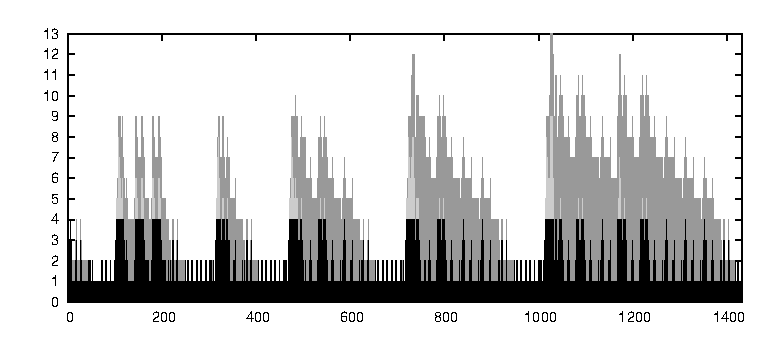
\includegraphics[width=12cm]{image/primes5_fullspec-threads.eps}

Thread Count

\noindent
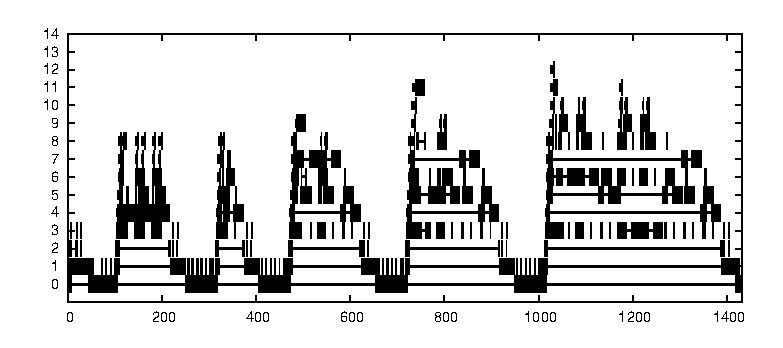
\includegraphics[width=12cm]{image/primes5_fullspec-activity.eps}

\caption{Profile of the evaluation of \texttt{(take 5 primes)} in fully speculative mode}
\label{figPrimesProfile}
\end{figure}


% ------------------------------------------------------------------------------------------------------- primes_source
\begin{figure}
\hrule
\medskip
\begin{verbatim}
primes          = primes'  $ from positiveInts 2;
primes' xx      = case xx of { (x:xs) -> x : primes' (sieve x xs); };

sieve   n xx    =
 case xx of {
        []      -> [];
        (x:xs)  -> if x % n == 0 then     sieve n xs
                   else               x : sieve n xs; };
\end{verbatim}
\hrule
\caption{\ample source for the \texttt{primes} function}
\label{figPrimesSource}
\end{figure}


The evaluation is driven by the \texttt{print} function which prints out the elements of the list one at a time. \texttt{print} makes use of the \texttt{seq} combinator to ensure that characters are output in the correct order. This results in obvious peaks in machine activity, corresponding to the $n$th prime number being evaluated, interspersed by periods of low activity when the values are printed out.

At the beginning of each iteration many threads are created. Although most of these threads become blocked straight away, the threads that finish their work become inactive and their indices are re-used. The visual activity in rows three and six in the thread count plot are the result of this behaviour. The alternative would be to increment the thread index for each new thread created, in a manner similar to \gransim's `per-thread activity profile' \cite{king:stratprof}, although this approach would become unwieldly with such a large number of fine grain threads. 

% The evaluation shown lasted 1386 steps, during which time 2607 reductions were performed and 3927 reductions were blocked. This corresponds to an average of 1.9 active threads over the entire evaluation. 

Figure\,\ref{figPrimesTally} shows a tally of how many times each reduction rule was invoked during the evaluation. Somewhat surprisingly, the rule used most frequently is \textbf{pe-var$3$/Cnstr} which updates the heap with a construct. On the other hand, the fact that the vast majority of reductions represent the `overhead' of lazy evaluation -- as opposed to operations on base types -- is less surprising.


\subsection{Explicitly parallel evaluation}
Figure\,\ref{figTreeProfile} shows the machine profile when evaluating an expression that inserts a list of elements into a binary tree and then determines the size of that tree. The expression evaluated was \mbox{\texttt{(parTreeSize tree)}} where the source for both \texttt{parTreeSize} and \texttt{tree} is shown in figure\,\ref{figTreeSource}. Although the tree is constructed in a sequential manner, \texttt{parTreeSize} creates a new thread to determine the number of elements in each branch. In this example 23 elements are inserted into the tree, though they are not all shown in the source. The communication latency has been set to 100 cycles.



% -------------------------------------------------------------------------------------------------- treeSize_profile
\begin{figure}

Thread Activity

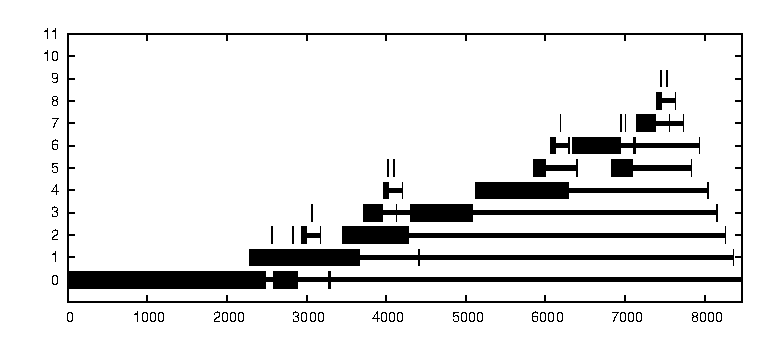
\includegraphics[width=12cm]{image/treeSize23_delay100-activity.eps}

Thread Count

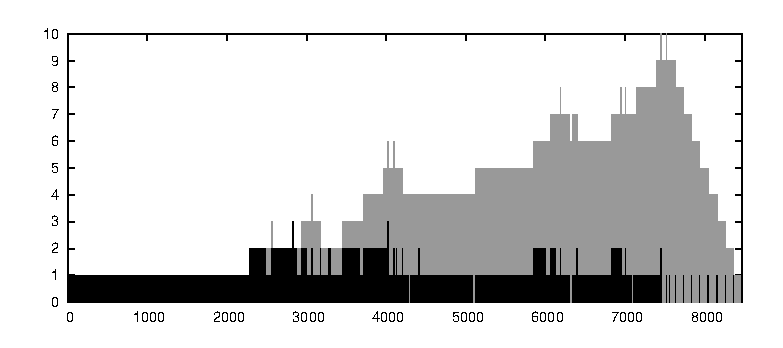
\includegraphics[width=12cm]{image/treeSize23_delay100-threads.eps}

Spawn Queue Length

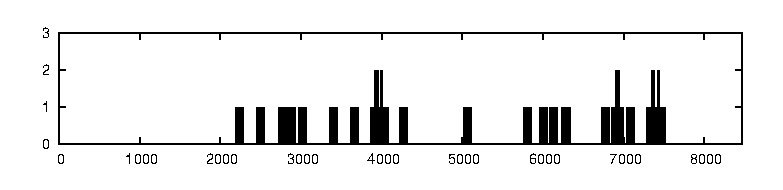
\includegraphics[width=12cm]{image/treeSize23_delay100-spawnQueueLength.eps}

Unblock Queue Length

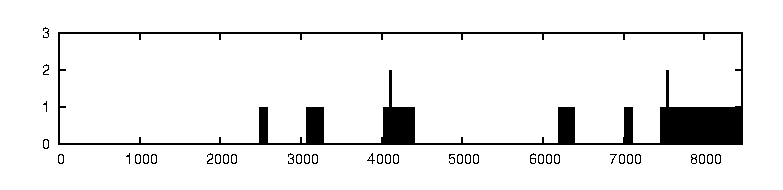
\includegraphics[width=12cm]{image/treeSize23_delay100-unblockQueueLength.eps}

\caption{Profile of the evaulation of \texttt{(parTreeSize tree)} with communication latency set to 100 cycles}
\label{figTreeProfile}
\end{figure}


% --------------------------------------------------------------------------------------------------------- primes_tally
\begin{figure}
\begin{tabular}{p{3cm}p{1cm}p{1cm}p{1cm}p{3cm}p{1cm}p{1cm}}
\toprule
\emph{Rule} 		& \emph{n}		& \emph{\%} 	& & \emph{Rule}		& \emph{n}	& \emph{\%}	\\
\cmidrule(r){1-3}\cmidrule(l){5-7}
pe-var3/Cnstr		& 450			& 0.17		& & prim/intEq		& 25		& 0.01		\\
pe-var1			& 338			& 0.13		& & seqPush		& 19		& 0.01		\\
app2			& 273			& 0.10		& & seqEval/Cnstr	& 19		& 0.01		\\
stop			& 272			& 0.10		& & prim/intMod		& 16		& 0.01		\\
fs-app1			& 271			& 0.10		& & prim/intAdd		& 11		& 		\\
case1			& 233			& 0.09		& & const/char		& 10		& 		\\
case2/match		& 232			& 0.09		& & print/char		& 10		& 		\\
pe-var3/Lambda		& 159			& 0.06		& & prim/intSub		& 7		& 		\\
let			& 139			& 0.05		& & print/int		& 5		&		\\
pe-var2			& 68			& 0.03		& & pe-app3		& 2		&		\\
const/int		& 47			& 0.02		& & case2/default	& 1		&		\\
\bottomrule
\end{tabular}
\caption{Tally of the number of times each reduction rule was taken during the evaluation of \texttt{(take 5 primes)}}
\label{figPrimesTally}
\end{figure}


% --------------------------------------------------------------------------------------------------- treeSize_source
\begin{figure}
\hrule
\medskip
\begin{verbatim}
treeInsert tree iKeyVal =
 case iKeyVal of {
    (iKey, iVal) ->
     case tree of {
        []                      -> (iKey, iVal, [], []);
        (key, val, left, right) ->
            if      iKey == key then KeyExists  
            else if iKey < key  then  
                 (key, val, treeInsert left iKeyVal, right)
            else (key, val, left, treeInsert right iKeyVal); }; };

parTreeSize tree =
 case tree of {
    []                      -> 0;
    (key, val, left, right) -> 
     let {
        sizeLeft    = parTreeSize left;
        sizeRight   = parTreeSize right;
     } in 
        sizeLeft par (sizeRight par (1 + sizeLeft + sizeRight)); };

elements    = ["perch", "barb", "tetra", "discus"   ... ]
elementIxs  = [5,       10,      4,      3          ... ]

tree = foldl treeInsert [] (zip elements elementIxs)
\end{verbatim}
\hrule
\caption{\ample source for the \texttt{parTreeSize} and \texttt{tree} functions}
\label{figTreeSource}
\end{figure}


As little work is done at the nodes of the tree the threads created for each branch quickly become blocked. From the profile we see that in the final stages of the reduction the number of active threads alternates between one and zero. This corresponds to the period where the sub-counts for each branch of the tree propagate back up to the main thread. As the threads corresponding to branches higher up in the tree have been blocked while waiting for lower threads to complete this information is carried by the machines unblocking mechanism. It takes 100 cycles for each of these values to be communicated and while this communication is taking place there is no other work to be done. This causes the number of active threads to fall to zero.

% ---------------------------------------------------------------------------------------------------------------- Related Work
\section{Related Work}
The \gransim\ series of profilers are run-time profilers for Glasgow Parallel Haskell (GpH) \cite{king:stratprof} \cite{loidl:thesis}. GpH is a mostly-implicit parallel extension of Haskell98 and makes use of the Glasgow Haskell Compiler (GHC) for the front end compilation while providing a new parallel run-time system named GUM \cite{gum-ifl}. \gransim\ comes in a number of flavours including \gransim-Lite which can be used to simulate an idealised machine with infinite processors and no communication cost.

The primary benefit that \ample has over \gransim\ and other such systems is that being an abstract machine, \ample it is much easier to modify and reason about. On the other hand, low level aspects such as graph packing techniques and caching strategies are beyond the scope of an abstract machine and are best left for such a system.


% ------------------------------------------------------------------------------------------------------------------ Conclusion
\section{Conclusion}
When working with an abstract machine, design ideas can be experimented with without the overhead of building a complete language implementation. We have seen that the careful analysis of the state transition rules given in \cite{baker-finch:sfp99} and \cite{sestoft:abstractmachine} has resulted in a modular system which provides useful information for small functions. Future work on \ample would allow the reduction rules take different numbers of steps so that machine behaviour closer to a native implementation could be simulated. \ample could also serve as the basis for an abstract machine for distributed processing. In such a machine, processing elements would consist of separate instances of the \ample abstract machine, connected by their existing IO mechanism.  


% ------------------------------------------------------------------------------------------------------------------ References
\bibliography{ample}
\bibliographystyle{plain}


% -------------------------------------------------------------------------------
\clearpage
\appendix{}

\section{AMPLE Reduction Rules}

\subsection{Rules for single threaded evaluation}

% ---------------------------------------
\rrule  {app$_1$}
	{ExpVar e x}	{[..., \px, ...]}	{S}		{H}
	{e}		{[..., \px, ...]}	{\px : S}	{H}
\medskip


% --------------------------------------
\rrule	{app$_2$}
	{Lambda e}	{E}			{\px : S}	{H}
	{e}		{\px : E}		{S}		{H}
\medskip


% --------------------------------------
\rrule	{var$_1$ (enter)} 
	{Var x}		{[..., \px, ...]}	{S}		{H [\px \bind (e', E') ]}
	{e}		{E'}			{\#{}\px : S}	{H}
\medskip	

% --------------------------------------
\rrule  {var$_2$ (update)}
        {\emph{whnf}}	{E}			{\#{}p : S}	{H}
	{\emph{whnf}}	{E}			{S}		{H [p \bind (\emph{whnf}, E')]}

\begin{tabular}{p{10mm}p{5mm}p{35mm}l}
	where	& E		& = [p$_0$, ... p$_a$, ... p$_n$] &
	\smallskip \\
		& E'		&    =    [p$_0$, \ldots p$_a$ \ldots p$_n$],	& when \emph{whnf} = Lambda e \\
		&               & $\;|\;$ [p$_0$, \ldots p$_a$],		& when \emph{whnf} = Cnstr m a \\
\end{tabular}
\medskip
	
%---------------------------------------
\rruleCfSE 
	{let}
	{Let [(b$_i$, t$_i$)] e$_0$ t$_0$}
	{E} 
	{S}
	{H}
	{e$_0$}	
	{E' $|$ t$_0$}
	{S}
	{H [p$_i$ $\rightarrow$ b$_i$, E' $|$ t$_i$ ]}	
\smallskip

\begin{tabular}{p{10mm}ll}
	where	& E'	& = [p$_n$, ... p$_1$] ++ E
\end{tabular}
\medskip


% --------------------------------------
\rruleCESfH	
	{case$_1$}
	{Case (e, t) alts}	{E}		{S}			{H}
	{e}			{E}		{(alts, E $|$ t) : S}	{H}
\medskip


% --------------------------------------
\rruleCESfH	
	{case$_2$}
	{Cnstr name$_i$ a$_i$}	{[p$_1$, ... p$_a$, ... p$_n$]}		{(alts, E) : S}	{H}
	{e$_i$}			{([p$_i$, ... p$_a$] ++ E) $|$ t$_i$}	{S}		{H}
\medskip


% --------------------------------------
\rruleCESfH
	{seqPush}
	{Seq e$_1$ e$_2$}	{E}		{S}			{H}
	{e$_1$}			{E}		{(SSeq e$_2$ E) : S}	{H}
\medskip


\newpage
% --------------------------------------
\rruleCESfH
	{seqEval}
	{\emph{whnf}}		{E}		{(SSeq e$_2$ E') : S}	{H}
	{e$_2$}			{E'}		{S}			{H}
\medskip


% --------------------------------------
\rruleCEfHS
	{constant\{Int$|$Char\}}
	{\{Int$|$Char\} v}	{E}				{S}	{H}
	{\{RetInt$|$RetChar\}}	{\{TagInt$|$TagChar\} : v : E}	{S}	{H}
\medskip


% --------------------------------------
\rruleCEfHS
	{print\{Int$|$Char\}}
	{PrimFunc ''print''}	{\{TagInt$|$TagChar\} : v : E}	{S}	{H}
	{Cnstr ''Done'' 0}	{E}				{S}	{H}
\medskip


% --------------------------------------
\rruleCEfHS	
	{prim\_intAdd}
	{PrimFunc IntAdd}	{TagInt : n1 : TagInt : n2 : E} {S}	{H}
	{RetInt}		{TagInt : (n1 + n2) : E}	{S}	{H}
\medskip
	
	
% --------------------------------------
\rruleCEfHS
	{prim\_intEq}
	{PrimFunc IntEq}	{TagInt : n1 : TagInt : n2 : E}	{S}	{H}
	{Cnstr \emph{name} 0}	{E}				{S}	{H}
\smallskip

\begin{tabular}{p{10mm}ll}
where	& \emph{name}	& = "True" $|$ "False"
\end{tabular}


% ----------------------------------------------------------------------------
\subsection{Modifications for parallel evaluation}

\rrule {pe-var$_1$ (enter)}
	{Var x}		{[..., \px, ...]}	{S}		{H [\px \bind (e, E)]}
	{e}		{E}			{\#{}\px : S}	{H [\px \bind \blockedon{[]}]}
\medskip

% --------------------------------------
\rrule {pe-var$_2$ (block)}
	{Var x}		{[..., \px, ...]}	{S}	{H [\px \bind \blockedon{ts}]}
	{\blocked}	{[ ]}			{S}	{H [\px \bind \blockedon{t:ts}]}
\medskip


% --------------------------------------
\noindent \textbf {pe-var$_3$ (unblock)}
\par
\medskip
\noindent
\begin{tabular} {p{ 5mm} p{ 5mm} p{8mm} p{20mm} p{15mm} p{ 8mm} p{50mm}}
	& ( 
	& \emph {whnf}, 
	& \raggedleft {[... \px, ...]},  
	& \raggedleft {\#{}\px : S}  
	& ) 
	& H [ \px \bind \blockedon{[t1, ...tn]} ]
	\\
	& \{(
	& \blocked,
	& \raggedleft{[ ]},
	& \raggedleft{S$_i$}
	& )$_i$ \}
	&
	\smallskip
	\\
	$\Rightarrow$	
	& (
	& \emph {whnf},
	& \raggedleft {[... \px, ...]},
	& \raggedleft {S}
	& )
	& H [ \px \bind (\emph {whnf}, [... \px, ...]) $_{[ ]}$ ]
	\\
	& \{(
	& \emph {whnf},
	& \raggedleft {[... \px, ...]},
	& \raggedleft {S$_i$}
	& )$_i$ \}
	&
	\\
\end{tabular}	
\smallskip

\begin{tabular}{p{10mm}ll}
where	& \emph{i} 	& = [t$_1$, ... t$_n$]		
\end{tabular}
\medskip

% -----------------------------------------------------------------------------
\subsection{Modifications for fully speculative evaulation}

\noindent \textbf {fs-app$_1$ (spawn)}
\par
\medskip
\noindent
\begin{tabular} {p{ 5mm} p{ 2mm} p{20mm} p{25mm} p{15mm} p{ 8mm} p{37mm}}
	& (
	& ExpVar e$_1$ x,
	& \raggedleft{[..., \px, ...]},
	& \raggedleft{S}
	& ) $_t$
	& H [\px \bind (e$_2$, E$_2$) ]
	\smallskip
	\\
	$\Rightarrow$
	& (
	& e$_1$,
	& \raggedleft{[..., \px, ...]},
	& \raggedleft{\px : S}
	& ) $_t$
	& H [\px \bind \blockedon{[ ]} ]
	\\
	& (
	& e$_2$,
	& \raggedleft{E$_2$},
	& \raggedleft{[ \#{}\px ]}
	& ) $_{t'}$
	\\
\end{tabular}
\smallskip

\begin{tabular}{p{10mm}ll}
where	& t'	& is fresh
\end{tabular}
\medskip


% --------------------------------------
\rrule	{fs-app$_3$}
	{ExpVar e x}	{[..., \px, ...]}	{S}		{H [\px \bind \blockedon{ts}]}
	{e}		{[..., \px, ...]}	{\px : S} 	{H}
\medskip


% -----------------------------------------------------------------------------
\subsection{Modifications for \texttt{par}-\texttt{seq} Evaluation}

\noindent \textbf {par-app$_1$ (spawn)}
\par
\medskip
\noindent
\begin{tabular} {p{ 5mm} p{ 2mm} p{20mm} p{25mm} p{15mm} p{ 8mm} p{37mm}}
	& (
	& Par x e$_1$,
	& \raggedleft{[..., \px, ...]},
	& \raggedleft{S}
	& ) $_t$
	& H [\px \bind (e$_2$, E$_2$) ]
	\smallskip
	\\
	$\Rightarrow$
	& (
	& e$_1$,
	& \raggedleft{[..., \px, ...]},
	& \raggedleft{\px : S}
	& ) $_t$
	& H [\px \bind \blockedon{[ ]} ]
	\\
	& (
	& e$_2$,
	& \raggedleft{E$_2$},
	& \raggedleft{[ \#{}\px ]}
	& ) $_{t'}$
	\\
\end{tabular}
\smallskip

\begin{tabular}{p{10mm}ll}
where	& t'	& is fresh
\end{tabular}
\medskip


% --------------------------------------
\rrule	
	{par-app$_2$}
	{Par x e$_1$}	{E}	{S}	{H [\px \bind \blockedon{[ ]}]}
	{e$_1$}		{E}	{S}	{H}
\medskip

% -----------------------------------------------------------------------------
%
%


\end{document}

